\chapter{Size Stream Measurement Definitions}
\section{Preface}

Definitions and images describing the standard measurements and landmarks from the Size Stream Scanner (Figure \ref{fig:SS scanner}) system used in this project are shown in the following pages. Terms and images sourced from Size Stream SS20 Measurements and Landmarks Definitions Version 2.0 March 24, 2019.

``Common terms used:

\begin{itemize}
    \item Contour circumference or measurement: Describes a measurement that follows the contours of the body part(s) being measured.
    \item Tape measurement: Describes a measurement that simulates a manual tape measure spanning the concave areas of the body parts(s) being measured.
    \item Point to Point distance: Describes a measurement that is the shortest distance from one measuring point to another. This measurement may go through the body.
    \item Height: All height measurements are “to the floor” unless specified otherwise.''
\end{itemize}

\begin{figure} [H]
    \centering
    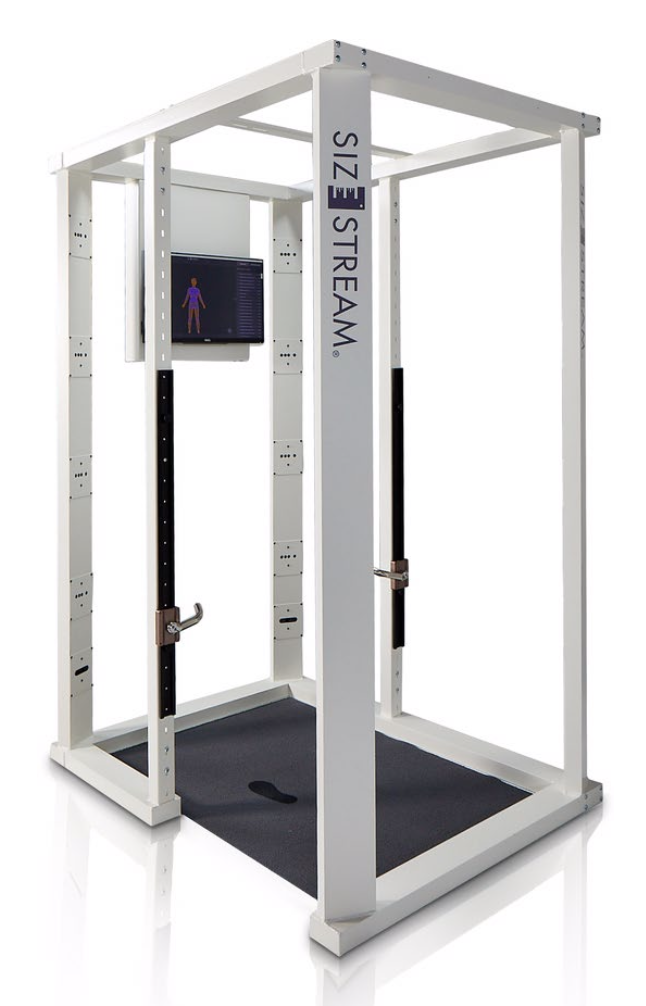
\includegraphics[width = 0.25\textwidth]{Images/SS scanner.png}
    \caption{Size Stream Scanner}
    \label{fig:SS scanner}
\end{figure}

\section{Measurements}
\begin{figure} [H]
    \centering
    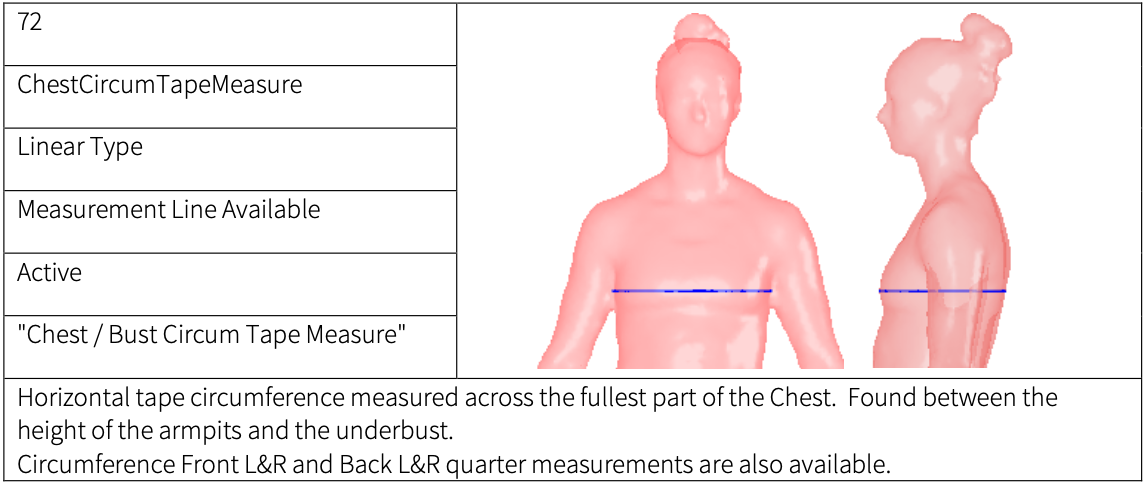
\includegraphics[width = 0.8\textwidth]{Images/ChestBustCircTM.png}
    \caption{Chest/Bust Circumference Tape Measure}
\end{figure}
\begin{figure} [H]
    \centering
    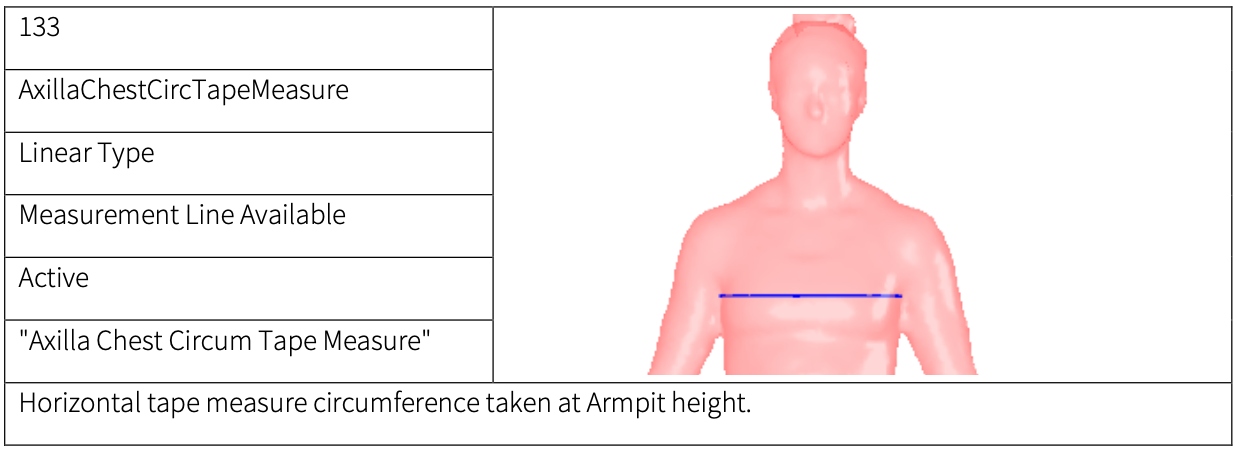
\includegraphics[width = 0.8\textwidth]{Images/AxillaCircTM.png}
    \caption{Axilla Chest Circumference Tape Measure}
\end{figure}
\begin{figure} [H]
    \centering
    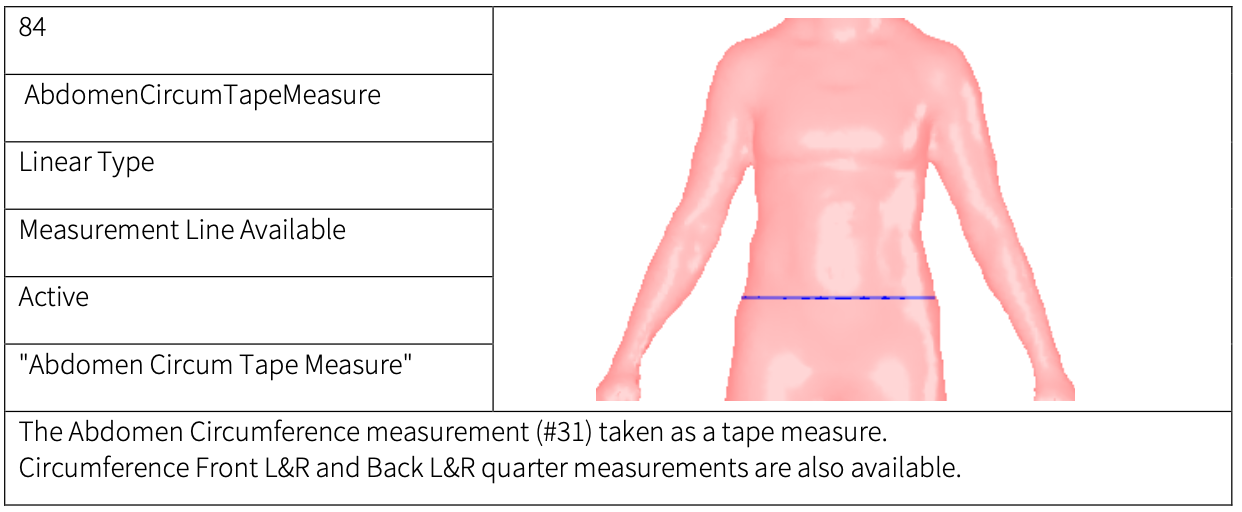
\includegraphics[width = 0.8\textwidth]{Images/AbdomenCircTM.png}
    \caption{Abdomen Chest Circumference Tape Measure}
\end{figure}
\begin{figure} [H]
    \centering
    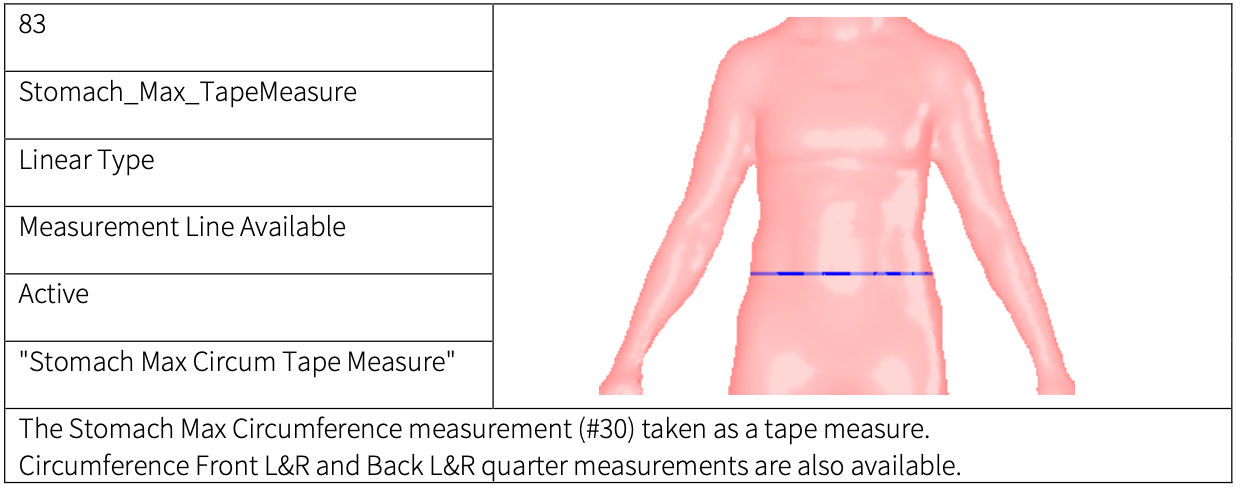
\includegraphics[width = 0.8\textwidth]{Images/StomachMaxTM.png}
    \caption{Stomach Max Circumference Tape Measure}
\end{figure}
\begin{figure} [H]
    \centering
    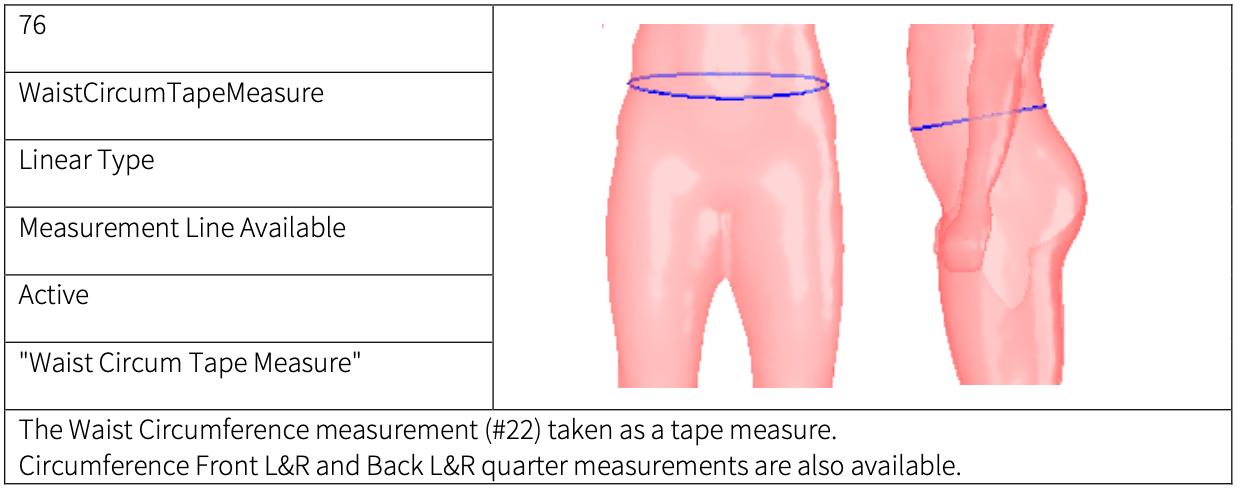
\includegraphics[width = 0.8\textwidth]{Images/Waist CircumTM.png}
    \caption{Waist Circumference Tape Measure}
\end{figure}
\begin{figure} [H]
    \centering
    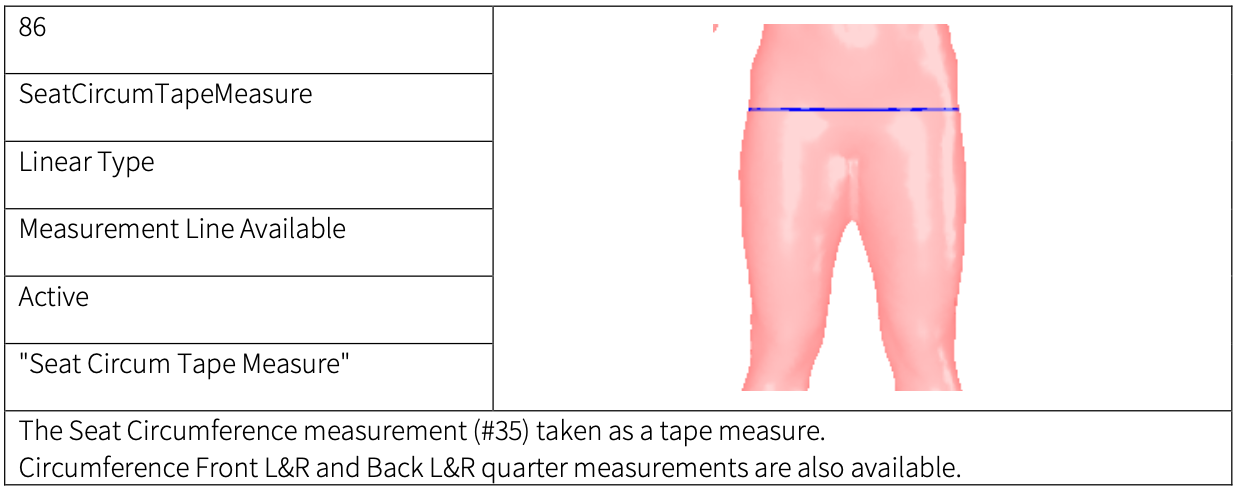
\includegraphics[width = 0.8\textwidth]{Images/SeatCircTM.png}
    \caption{Seat Circumference Tape Measure}
\end{figure}
\begin{figure} [H]
    \centering
    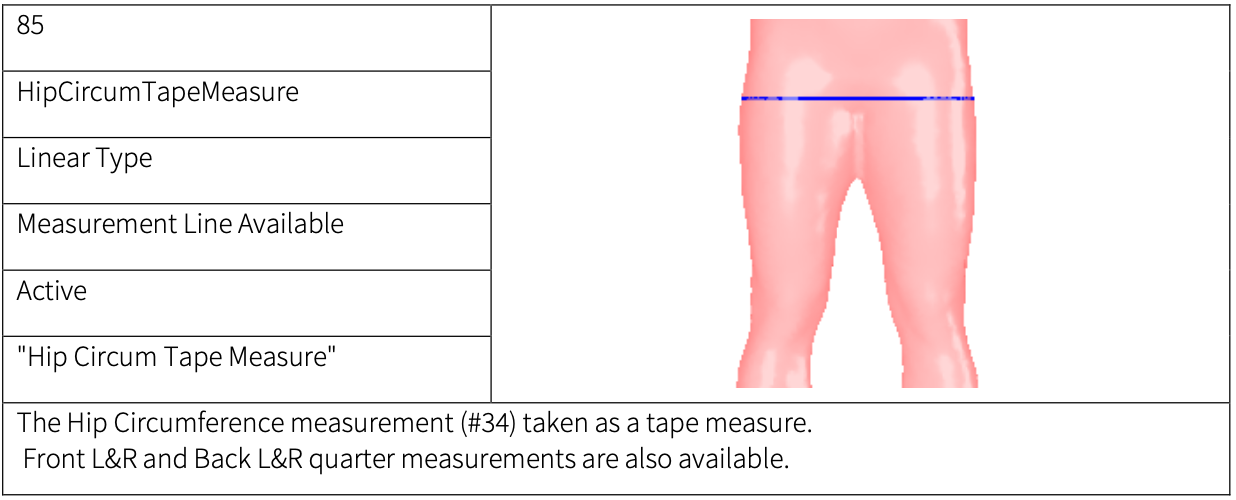
\includegraphics[width = 0.8\textwidth]{Images/HipCircTM.png}
    \caption{Hip Circumference Tape Measurement}
\end{figure}
\begin{figure} [H]
    \centering
    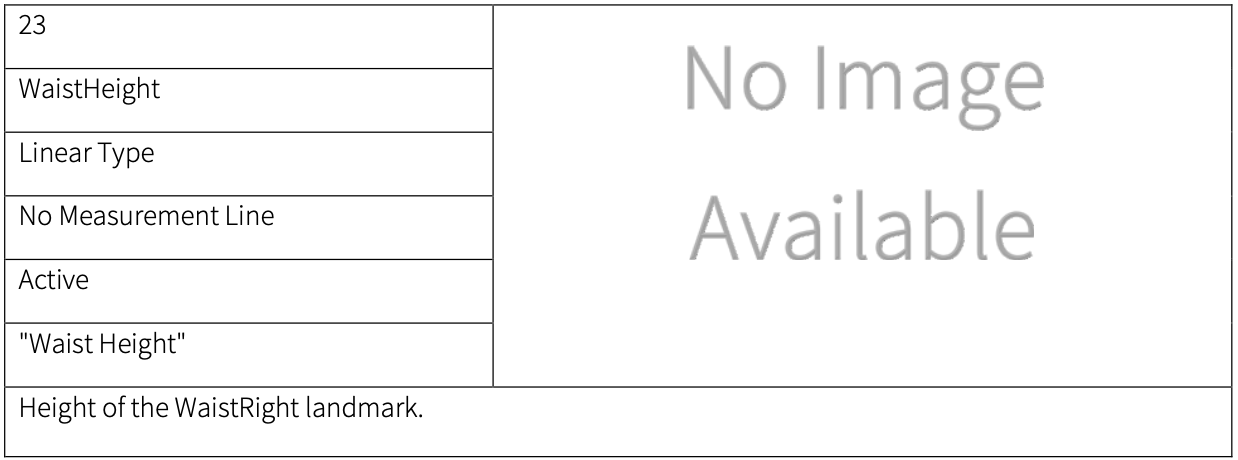
\includegraphics[width = 0.8\textwidth]{Images/WaistHeight measurment.png}
    \caption{Waist Height}
\end{figure}
\begin{figure} [H]
    \centering
    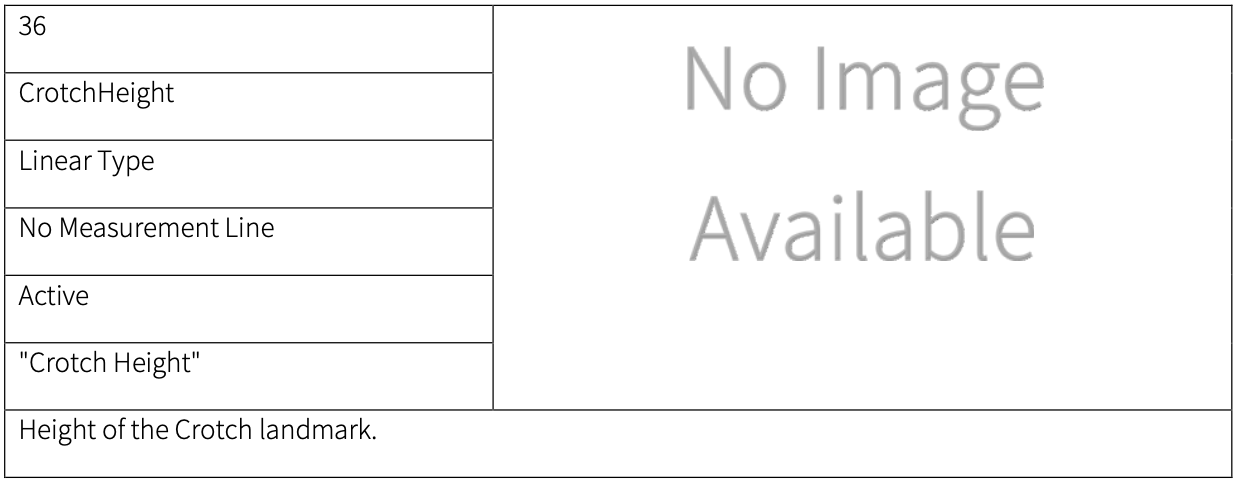
\includegraphics[width = 0.8\textwidth]{Images/CrotchHeight measurment.png}
    \caption{Waist Height}
\end{figure}

\section{Landmarks}
\begin{figure} [H]
    \centering
    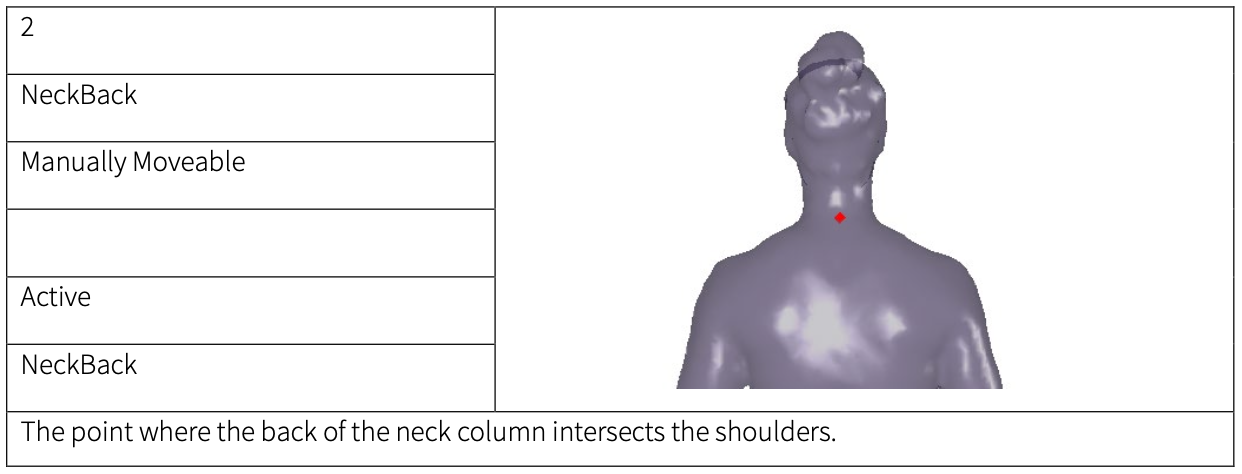
\includegraphics[width = 0.8\textwidth]{Images/NeckBack landmark.png}
    \caption{Neck Back Landmark}
\end{figure}
\begin{figure} [H]
    \centering
    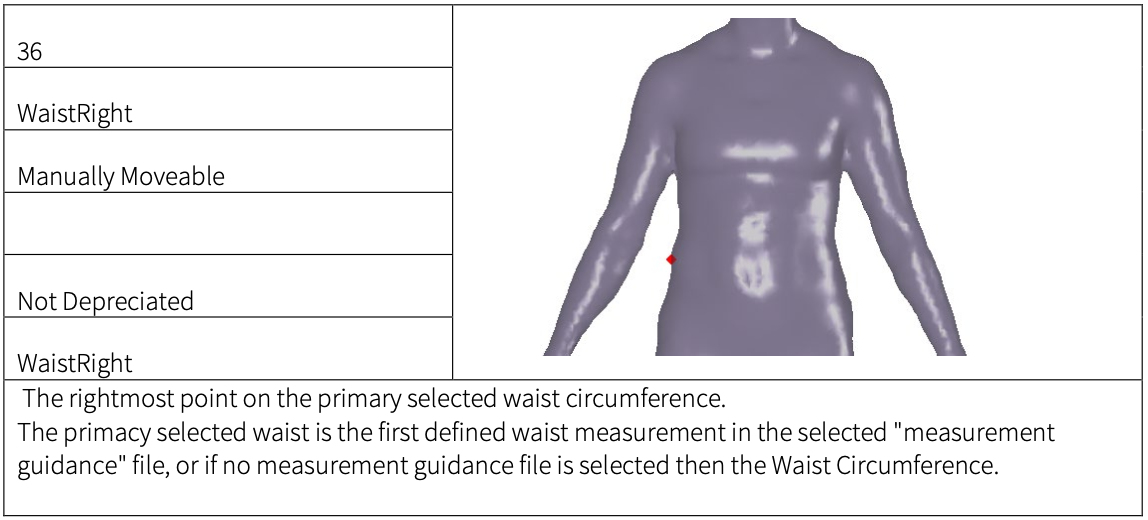
\includegraphics[width = 0.8\textwidth]{Images/WaistRight landmark.png}
    \caption{WaistRight Landmark}
\end{figure}
\begin{figure} [H]
    \centering
    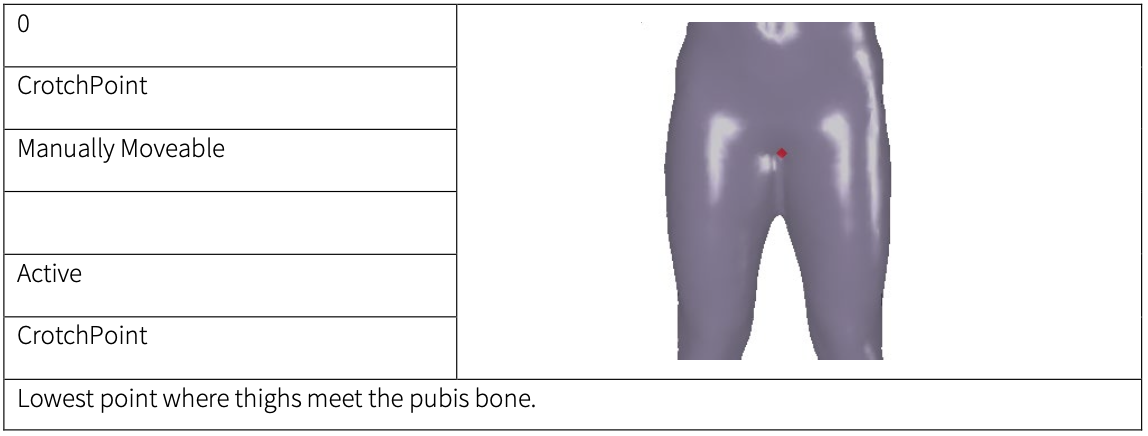
\includegraphics[width = 0.8\textwidth]{Images/CrotchPoint landmark.png}
    \caption{Waist Height}
\end{figure}
